\apendice{Especificación de diseño}

\section{Introducción}
En este apartado se describe cómo se ha diseñado la aplicación \emph{SurveyingPointCode} para cumplir con los objetivos y las especificaciones definidas anteriormente.

Se definen los datos a utilizar por la aplicación así como el diseño procedimental y su arquitectura.
\section{Diseño de datos}

Las entidades de esta aplicación están enfocadas a la generación de un dibujo final. A continuación se describe cuales son y como se relacionan entre ellas. 


\begin{itemize}

\item \textbf{Dibujo:} Almacena todos los elementos que componen el dibujo, tanto geométricos, como no geométricos. Está compuesto por: un nombre, capas, puntos y textos. De forma opcional puede contener: líneas, \emph{splines}, círculos y símbolos.

\item \textbf{Capa:} Todos los elementos del dibujo se guardan en capas. Está compuesto por: un nombre y un color.

\item \textbf{Punto:} Elemento básico del dibujo. Está compuesto por: un número, una coordenada $X$, una coordenada $Y\!$, una coordenada $Z$, un código y una capa.

\item \textbf{Línea:} Formada por una lista de puntos. Está compuesto por: una lista de puntos y una capa.

\item \textbf{\emph{spline}:} Formada por una lista de puntos. Está compuesto por: una lista de puntos y una capa.

\item \textbf{Círculo:} Está compuesto por: un punto, un radio y una capa.

\item \textbf{Bloque:} Elemento interno de CAD que almacena un símbolo. Está compuesto por: un nombre, un punto y una capa.

\item \textbf{Texto:} Texto asociado a un punto, en este caso pude ser, el número del punto, su altitud o su código. Está compuesto por: un punto, el tamaño del texto, el desplazamiento con respecto al punto, el texto y una capa.

\end{itemize}

Aunque no se ha implementado como una base de datos, la relación entre los elementos dentro de la biblioteca \texttt{ezdxf}, se comporta de la misma forma.

A continuación se puede ver el diagrama relacional. Se ha representado en dos diagramas para facilitar su comprensión (en un mismo diagrama saldrían líneas superpuestas y sería muy confuso de interpretar).

En la Figura~\ref{fig:DR-1}, se ven las relaciones de todos los elementos con el elemento principal, el dibujo.

\begin{figure}[H]
	\centering
	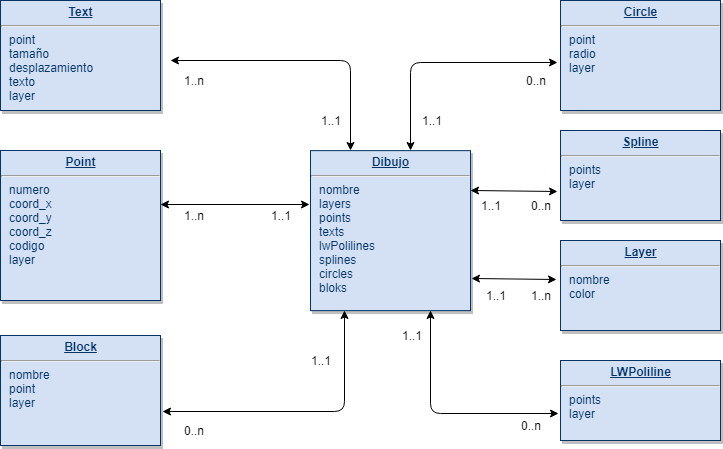
\includegraphics[width=0.9\textwidth]{DR-1}
	\caption{Diagrama relacional principal.}
	\label{fig:DR-1}
\end{figure}

En la Figura~\ref{fig:DR-2}, se ven las relaciones entre sí, del resto de elementos.

\begin{figure}[H]
	\centering
	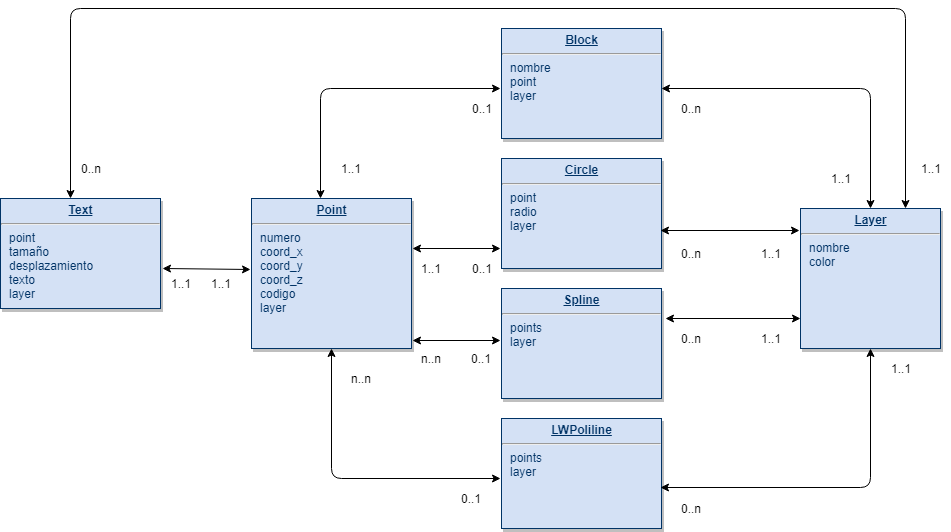
\includegraphics[width=1\textwidth]{DR-2}
	\caption{Diagrama relacional elementos del dibujo.}
	\label{fig:DR-2}
\end{figure}

\section{Diseño arquitectónico}

Como se ha detallado en la memoria (ver apartado 4.2. Patrones de diseño), para el diseño de la aplicación se ha utilizado el patrón arquitectónico \textbf{MTV}, que es similar al MCV, pero con alguna diferencia. \textbf{T} significa \emph{Template}, plantilla, que son los datos que se presentan al usuario y \textbf{V} significa vista, la capa de la lógica de negocios.
\textbf{MTV} es la arquitectura usada por \texttt{Flask}. 


\begin{figure}[H]
	\centering
	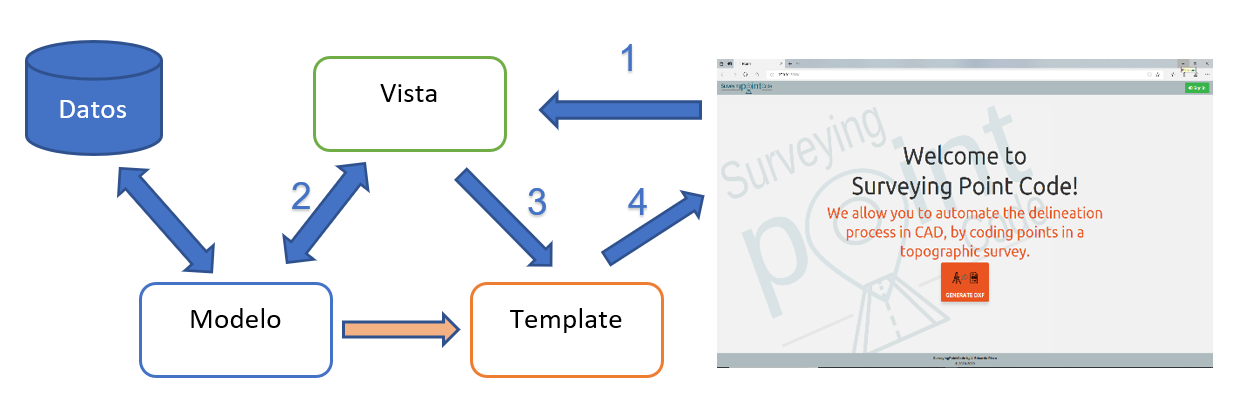
\includegraphics[width=0.5\textwidth]{MTV}
	\caption{Esquema de un patrón MTV.}
	\label{fig:MTV}
\end{figure}
Como sistema de base de datos se ha utilizado \textbf{PostGIS}. Para tener más independencia de la base de datos se ha optado por usar un \textbf{ORM}, \emph{SQLALchemy}. El uso de un ORM,  simplificará el desarrollo y si en un futuro se decide cambiar de base de datos, será mas sencilla la adaptación de la aplicación.


\begin{figure}[H]
	\centering
	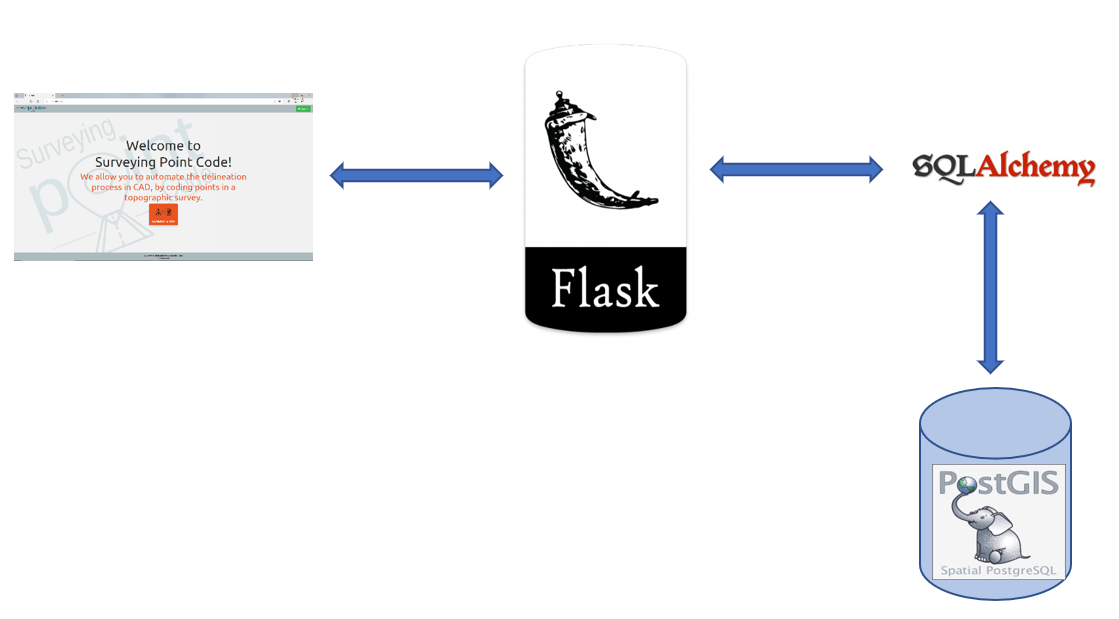
\includegraphics[width=0.5\textwidth]{Arq_1}
	\caption{Diseño arquitectónico con ORM y BBDD.}
	\label{fig:Arq_1}
\end{figure}

La aplicación se ha terminado de construir utilizando el sistema de contenedores \emph{Docker}. Con el uso de esta infraestructura se mejora la capacidad de ejecutar varios procesos y aplicaciones por separado y, al mismo tiempo, también conserva la seguridad que tendría con sistemas separados. Los contenedores \emph{Docker} son una especie de máquinas virtuales, pero más ligeras, que permiten  encapsular cualquier arquitectura, convirtiéndola en un contenedor portable y autosuficiente. 


\begin{figure}[H]
	\centering
	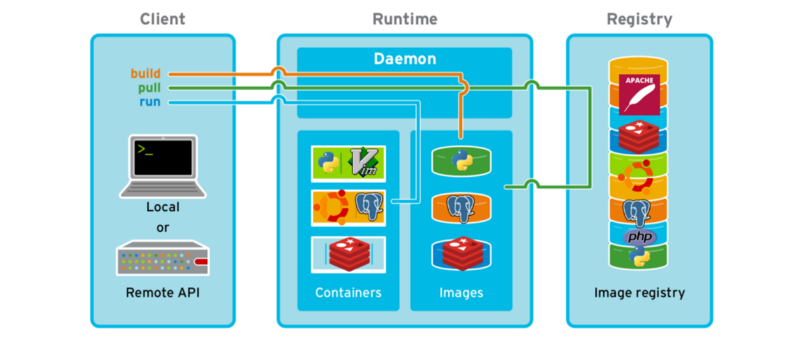
\includegraphics[width=0.7\textwidth]{Arq_docker}
	\caption[Arquitectura de \emph{Docker}]{Arquitectura de \emph{Docker}~\cite{arq_dock}.}
	\label{fig:Arq_docker}
\end{figure}

\noindent como se puede ver en la imagen anterior, \emph{Docker} está compuesto por tres partes:

\begin{itemize}
\item \emph{Docker client}: herramienta en línea de comandos, responsable para comunicarnos con el servidor \emph{Docker}. La comunicación se lleva a cabo mediante una \emph{RESTful API} a la cual solicitamos operaciones.

\item \emph{Docker Runtime}: este servicio, que se ejecuta como un demonio en un sistema operativo, construye, ejecuta y descarga las imágenes de los contenedores. El demonio puede ejecutarse en el mismo sistema que el cliente \emph{Docker} o de forma remota.

\item \emph{Docker Registry}: aquí se almacenan imágenes para uso público o privado. El conocido registro público es \emph{Docker Hub}, y almacena múltiples imágenes desarrolladas por la comunidad. Existe también la posibilidad de crear registros privados.

\end{itemize}

La arquitectura final basada en \emph{Docker} que se ha implementado, queda de la siguiente forma:

\begin{itemize}

\item \textbf{\emph{API Flask}}: contiene la aplicación desarrollada en \emph{Flask} y esta conectado con el contendedor \emph{PostGIS}.

\item \textbf{\emph{PostGIS}}: contiene la base de datos y esta conectado con los contendedores \emph{API Flask} y \emph{PgAdmin}.

\item \textbf{\emph{PgAdmin}}: contiene la aplicación \emph{PgAdmin 4}, para la gestión de la base de datos y esta conectado con el contendedor \emph{PostGIS}.
\end{itemize}

\begin{figure}[H]
	\centering
	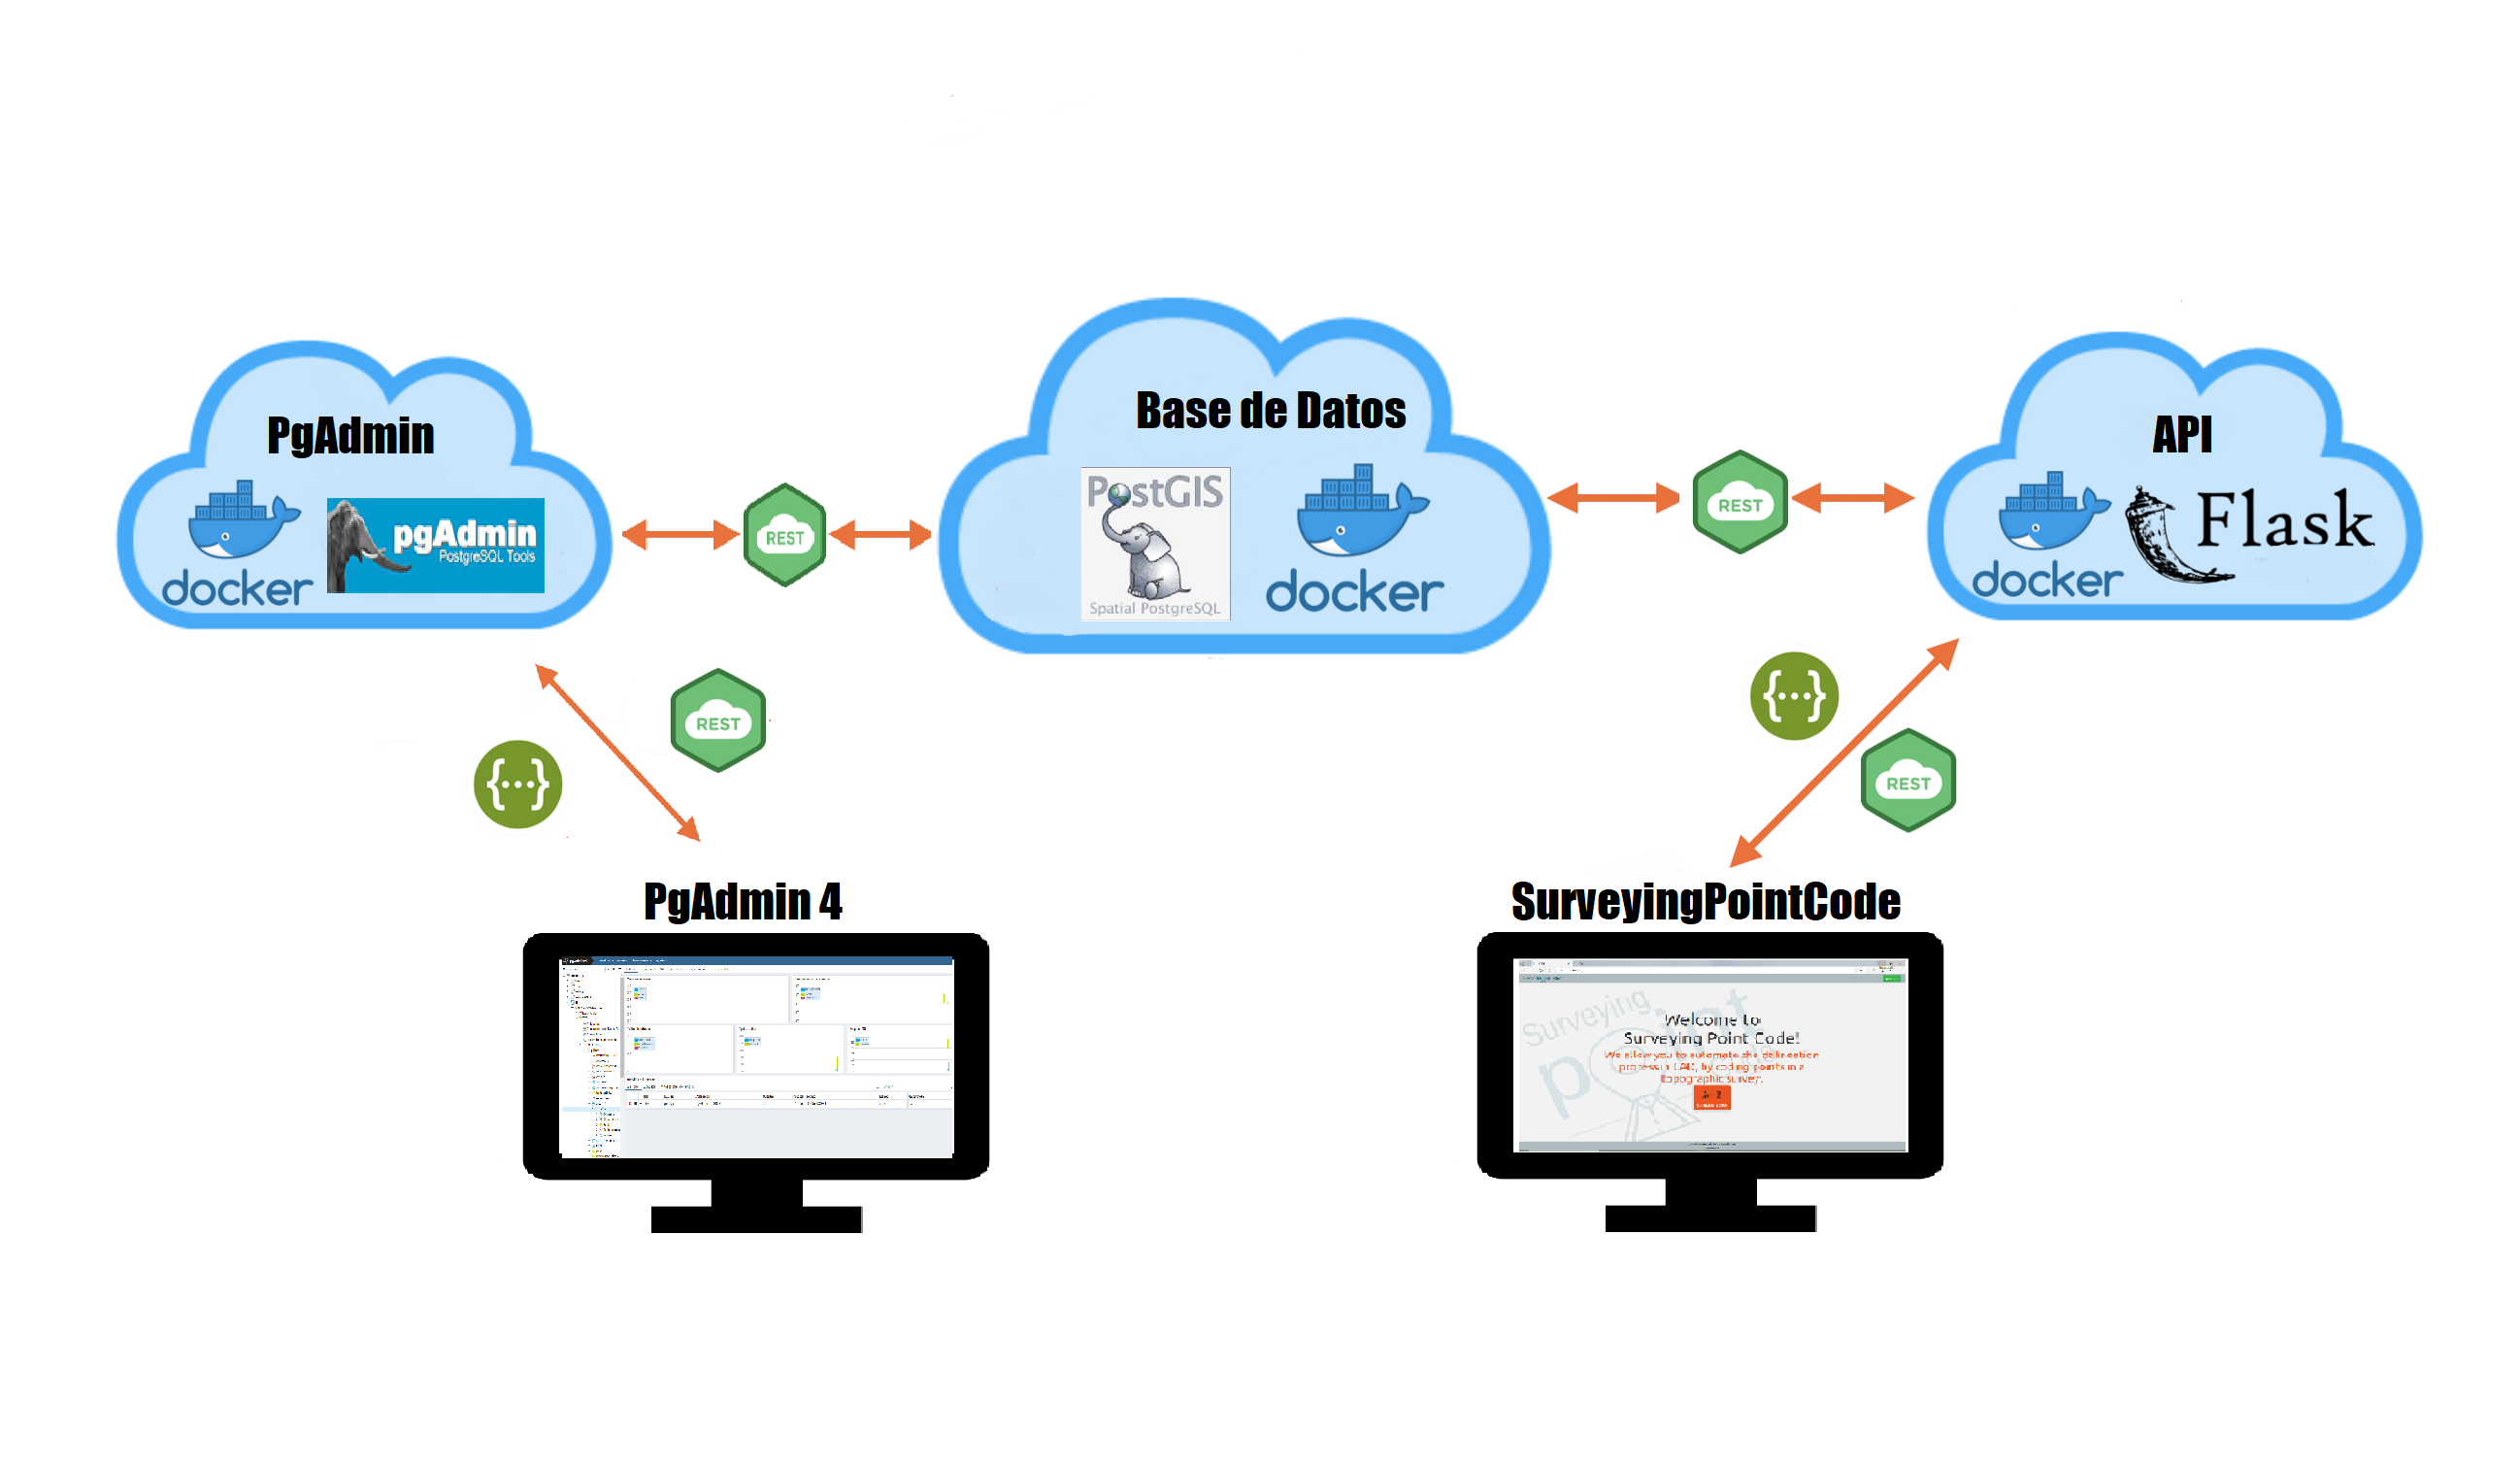
\includegraphics[width=1\textwidth]{Arq_SPC}
	\caption{Arquitectura final de la aplicación con \emph{Docker}}
	\label{fig:Arq_SPC}
\end{figure}

\section{Diseño procedimental}

En este apartado se presenta la especificación procedimental del algoritmo utilizado en forma de diagrama de flujo y diagrama de secuencia de la aplicación.


\begin{figure}[H]
	\centering
	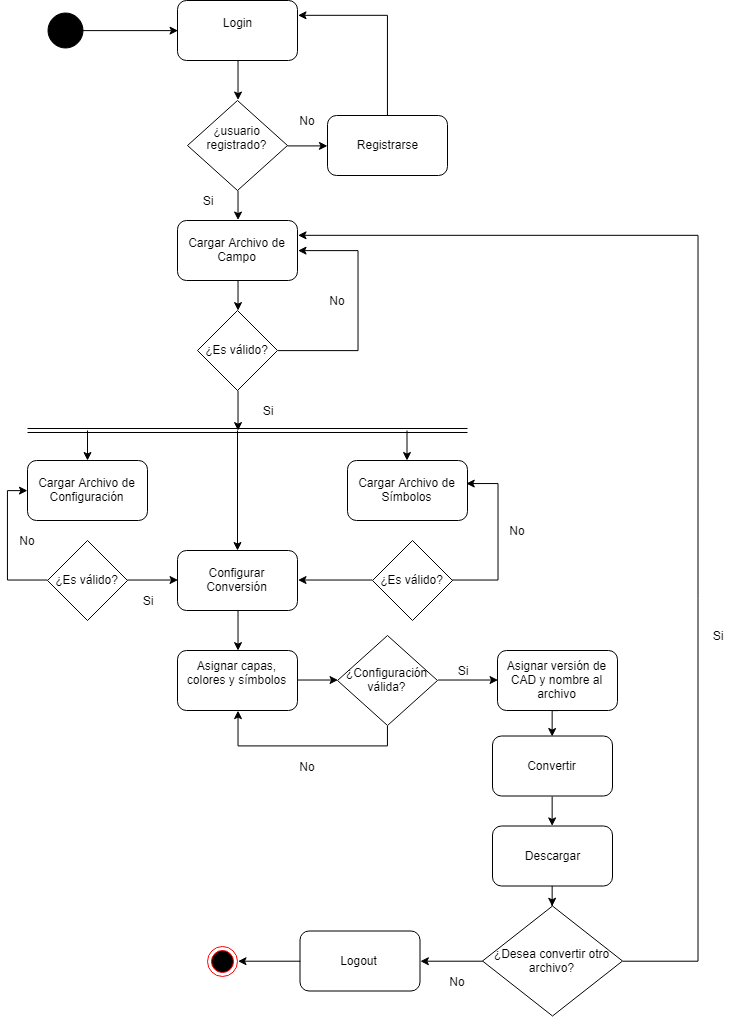
\includegraphics[width=0.8\textwidth]{D_Flujo}
	\caption{Diagrama de flujo de la aplicación}
	\label{fig:D_Flujo}
\end{figure}

\begin{figure}[H]
	\centering
	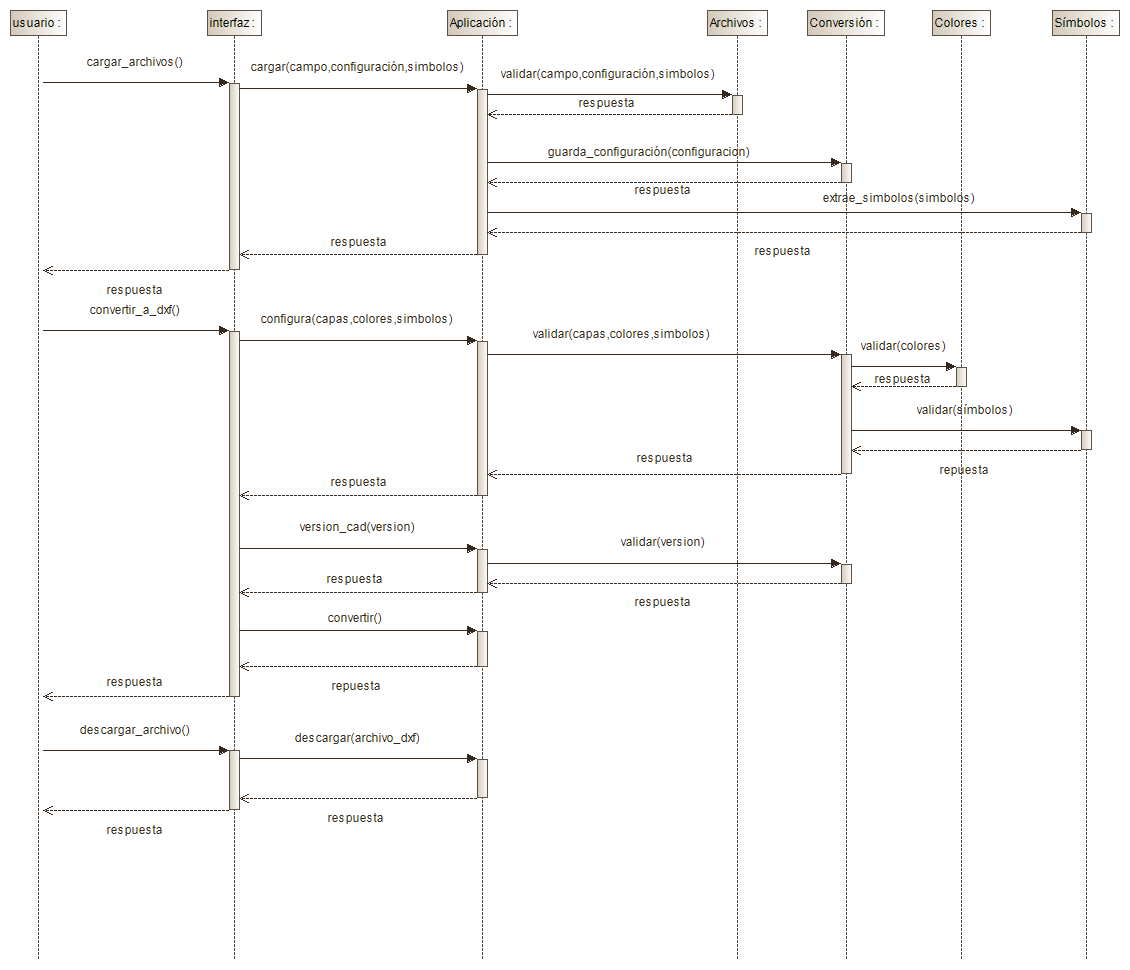
\includegraphics[width=1\textwidth]{DS_4}
	\caption{Diagrama de secuencia general}
	\label{fig:DS_4}
\end{figure}